

\chapter { Etude préliminaire du projet }


\section*{Introduction}
\addcontentsline{toc}{section}{Introduction}
\bigskip
Dans le cadre de la mise en place d'une application de gestion des parking des entreprises, il est essentiel de réaliser une étude préalable approfondie afin de cerner les besoins, les contraintes et les objectifs liés à ce projet. Cette étude préalable permettra de définir les contours du projet et de poser les bases pour son développement et sa mise en œuvre.
Nous commençons par placer le projet dans son cadre général et d'exposer le contexte de travail ainsi que  les objectifs a atteindre.

%_________________________________________________________________________________________________

\section{Présentation de l’organisme d’accueil}
\bigskip
Digital Identity, connue sous l’abréviation « DIGID »est une entreprise tunisienne Fondée en 2019, spécialisée dans le conseil et le développement de solutions technologiques spécifiques à l'échelle nationale et internationale. Ses objectifs sont de permettre à ses clients de se concentrer sur leurs activités principales, en s'appuyant sur des solutions fiables et sur un partenaire crédible et inébranlable.\\
\newline DIGID est spécialisée dans le conseil et la mise en œuvre de solutions logicielles de gestion intégrée.

\bigskip
\begin{figure}[ht]
    \centering
    
\includegraphics[scale = 0.5]{chap1.images/digidlogo.png}
    \caption{Logo de l’entreprise « DIGITAL IDENTITY »}
    \label{Logo de l’entreprise « DIGITAL IDENTITY » }
\end{figure}

%____________


\newpage
\subsection{ Organigramme de l’entreprise }

L’organigramme de Digital Identity figure 1.2 présente une vue parfaite de l’oraganisation des
liens hiéarchiques entre les différentes équipes. En effet, c’est une traduction schématique des
objectifs, des missions et des relations fonctionnelles.

\begin{figure}[ht]
    \centering
    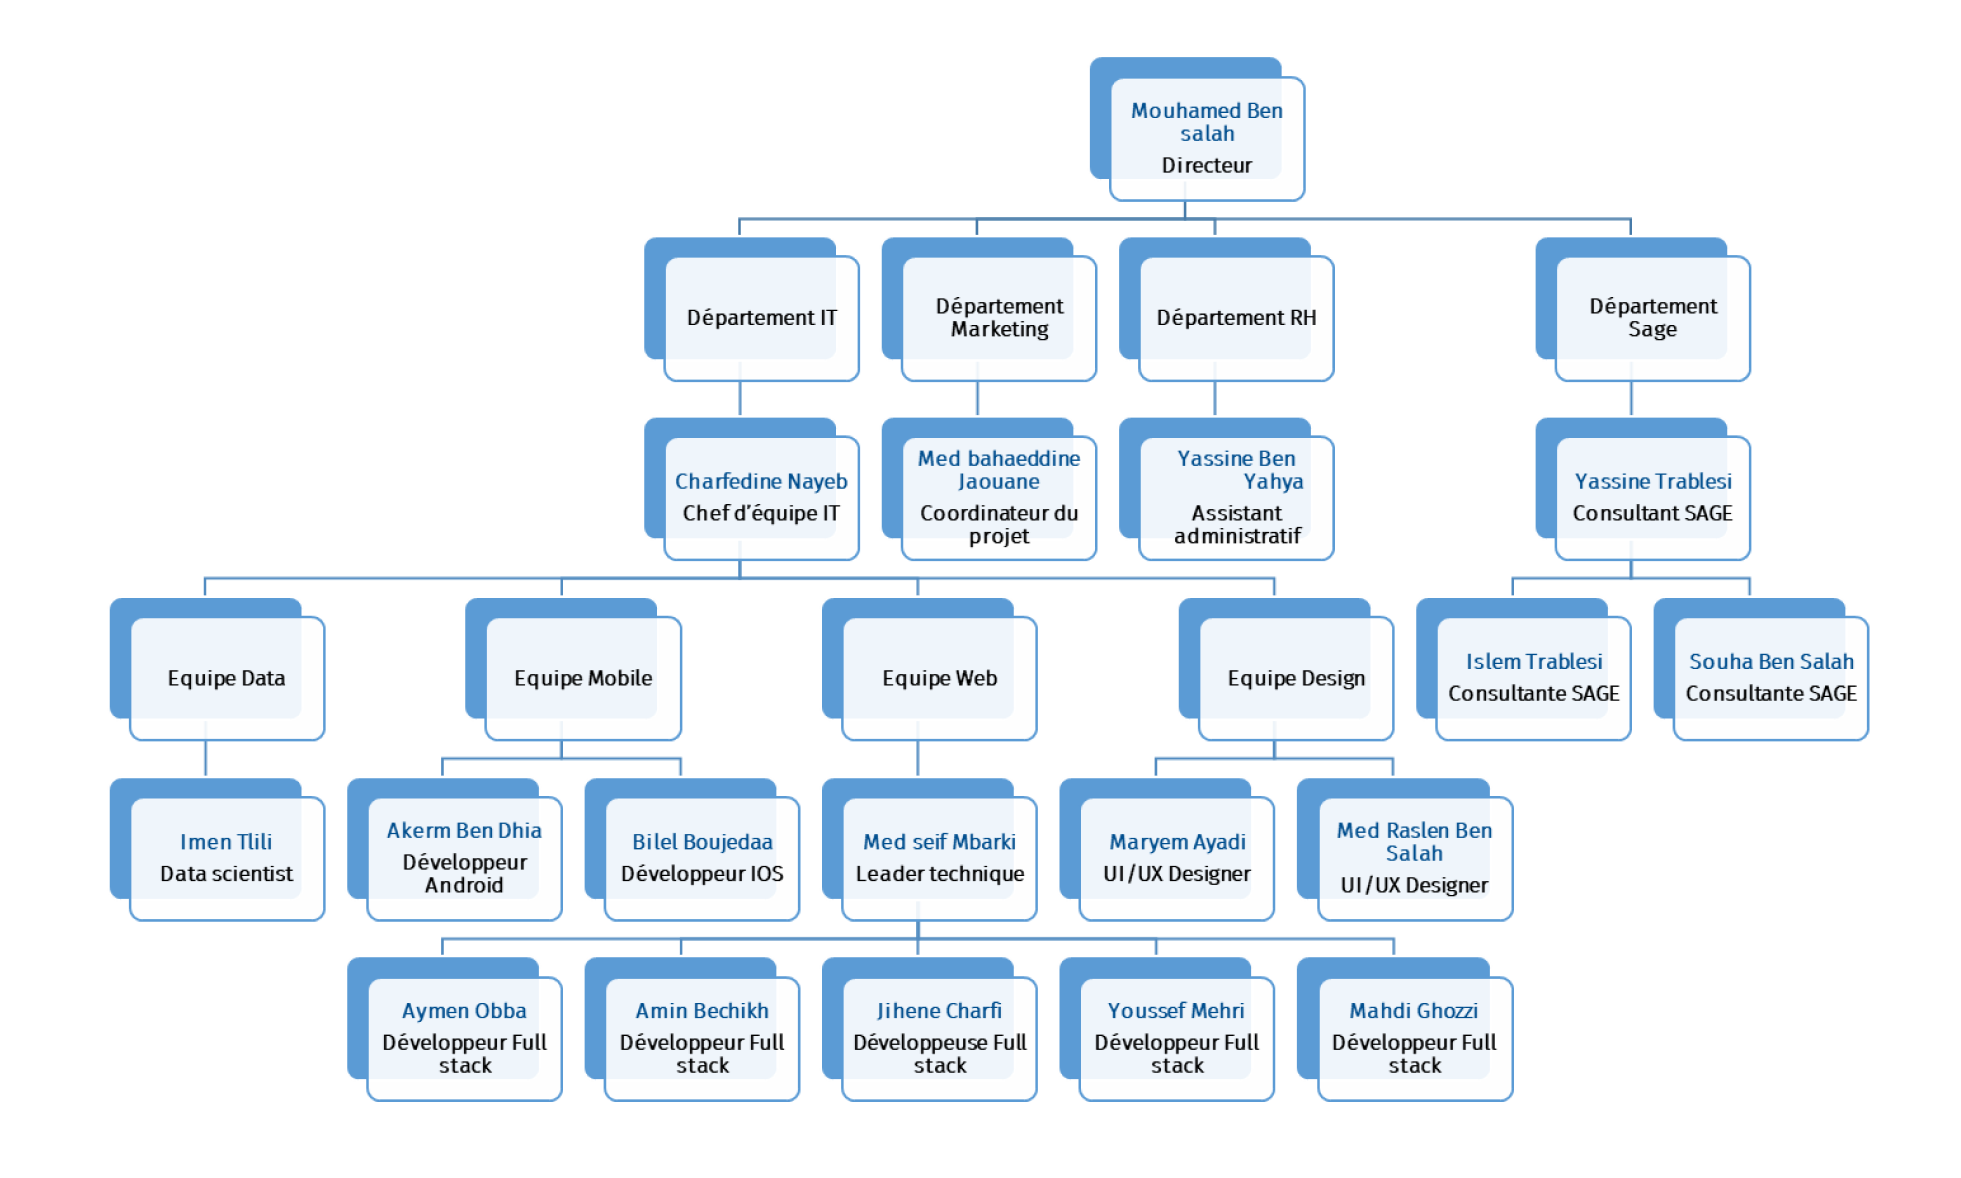
\includegraphics[width=1.1\textwidth,height=12.5cm]{chap1.images/org digid.png}
    \caption{Organigramme de Digital identity}
    \label{fig:orgcogecom}
\end{figure}


\subsection{ Les activités de Digital Identity : }
\begin{figure}[ht]
    \centering
    \includegraphics[width=1\textwidth,height=4cm]{chap1.images/digid activités.png}
    \caption{Les activités de Digital Identity}
\end{figure}
%_________________________________________________________________________________________________
\newpage
\section{Cadre du projet}
\bigskip
Dans cette section, nous allons aborder en détail la problématique soulevée et nous allons présenter une solution pertinente qui a été proposée pour y remédier.
\bigskip
\subsection{ Problématique}
\bigskip
À une époque où la gestion des parcs de véhicules d'entreprise est devenue de plus en plus complexe en raison de la diversité des véhicules, des itinéraires et des exigences opérationnelles, ainsi que des pressions technologiques et environnementales croissantes, il devient impératif de concevoir, développer et déployer une plateforme intégrée véritablement innovante et robuste pour relever ces défis multidimensionnels. Comment mettre en place une telle plateforme, capable de fournir une surveillance en temps réel, une analyse prédictive et des fonctionnalités d'optimisation avancées, tout en garantissant une efficacité opérationnelle maximale, une réduction des coûts et une durabilité environnementale accrue pour les entreprises? De plus, comment concilier ces objectifs avec les exigences de sécurité, de conformité réglementaire et de flexibilité, afin de permettre aux entreprises de prospérer dans un contexte économique en perpétuelle mutation, de maintenir leur compétitivité et d'assurer une gestion stratégique de leurs actifs de transport dans un monde en constante évolution ?



%_________________________________________________________________________________________________

\subsection{ Solution proposée}
\bigskip
Notre solution de gestion de flotte de véhicules d’entreprise repose sur une plateforme intégrée et technologiquement avancée, conçue pour répondre aux défis croissants de gestion des parcs de véhicules. Dans le cadre de cette solution, nous avons intégré une dimension Business Intelligence (BI) afin d'offrir une analyse approfondie des données et des informations stratégiques aux gestionnaires. Cette intégration du volet BI enrichit notre plateforme en lui permettant de fournir une surveillance en temps réel des véhicules, une analyse prédictive des données et des outils d'optimisation avancés.

Grâce à des tableaux de bord interactifs et des rapports personnalisables, les gestionnaires auront une vue d'ensemble précise de la performance opérationnelle de leur flotte. Ces outils leur permettront de visualiser et de suivre en temps réel des indicateurs clés de performance (KPI) tels que le taux d'utilisation des véhicules, les coûts de maintenance, les temps d'immobilisation, etc. De plus, les rapports générés par le système BI fourniront des insights stratégiques pour la prise de décision, en identifiant les tendances, les patterns et les opportunités d'optimisation.

En combinant ces fonctionnalités avancées avec une approche centrée sur les besoins des entreprises, notre solution vise à fournir une réponse complète et efficace aux défis de gestion des flottes de véhicules d’entreprise. Elle permettra aux gestionnaires de prendre des décisions éclairées et proactives pour maximiser l'efficacité opérationnelle de leur flotte, réduire les coûts associés et maintenir leur compétitivité dans un environnement commercial en constante évolution.


%______________________________________________________________________________________________




\section{Méthodologie et langage de conception}
La conception est cruciale dans le développement d'un système informatique pour répondre aux besoins du client. Les choix conceptuels concernant l'approche, le langage de modélisation et le processus de développement sont issus de réflexions collectives. Nous avons choisi la méthodologie Scrum, une méthode agile, pour réaliser notre projet.
\subsection { Méthodes agiles}
\noindent Parmi les méthodes agiles les plus couramment utilisées de nos jours, on peut citer :

\begin{itemize}[label=$\square$]
    \item Extrême Programming (XP)
    \item Scrum
    \item Agile Unified Process (Agile UP ou AUP)
\end{itemize}


Ces méthodes agiles se caractérisent par leur approche itérative et incrémentale, leur focalisation sur les besoins des utilisateurs, leur flexibilité pour répondre aux changements, leur collaboration étroite avec les parties prenantes du projet, ainsi que leur orientation vers une livraison régulière de fonctionnalités à valeur ajoutée. Chacune de ces méthodes agiles a ses propres pratiques, rôles, cérémonies et outils, mais elles partagent toutes les mêmes valeurs et principes fondamentaux de l'agilité.\\

Dans notre cas ,nous avons choisi d'adopter le framework Scrum pour le développement de notre application, car elle nous a semblé la plus adaptée à notre travail. Scrum est un framework agile qui offre une organisation flexible nous permettant de découper notre projet en plusieurs sprints. Cette approche itérative nous aidera à mieux gérer notre travail en nous concentrant sur des objectifs concrets à atteindre à chaque étape du développement.


%_________________________________________________________________________________________________


\newpage
\subsection{ Principes du framework Scrum}
Scrum est un cadre de travail pour la gestion de projet agile qui est largement utilisé à travers le monde. Il comprend des rôles bien définis, un rythme itératif, des réunions chronométrées et des artefacts tels que le product backlog, le sprint backlog et le graphique d'avancement (Burndown Chart). Ces éléments constituent les piliers du processus de gestion de projet agile offert par Scrum.\\

\begin{figure}[htbp]
    \centering
    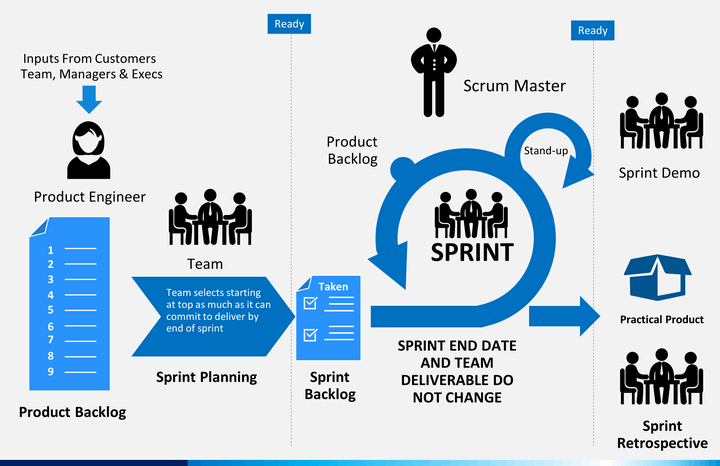
\includegraphics[width=1\textwidth]{chap1.images/scrum-process-slide2_2.png}
    \caption{Mode de fonctionnement de la méthodologie Scrum}
\end{figure}

\noindent\textbf{Sprint} : Tout projet Scrum est organisé autour de «Sprints» de développement pendant lesquels une équipe de développement travaille sur un ensemble de fonctionnalités ou d'objectifs spécifiques.

\noindent\textbf{User story} : Les fonctionnalités requises sont présentées sous la forme de "User Stories" dans une liste organisée.

\noindent\textbf{Backlog du produit} : Les user stories sont organisées dans le backlog du produit.\\

\noindent\textbf{Sprint backlog} : Le sprint backlog est une liste des éléments du product backlog sélectionnés pour être développés pendant un sprint exacte. C'est une liste de tâches à accomplir pendant le sprint. Les membres de l'équipe de développement se concentrent sur ces tâches pour les livrer à la fin du sprint.

\noindent\textbf{Planning pocker} : Pendant une réunion nommée "Réunion du Planning Poker", les user stories de chaque sprint sont estimées en points et priorisées.

\noindent\textbf{La mêlée quotidienne} : La mêlée quotidienne permet aux membres de l'équipe de se synchroniser régulièrement, de signaler rapidement les problèmes et les défis qu'ils rencontrent et de suivre l'avancement du sprint en temps réel. Cette réunion rapide et efficace est un moyen pour l'équipe de travailler de manière collaborative et d'assurer la réussite du projet.

\noindent\textbf{Revue de sprint} : L’objectif de la revue de sprint est d’inspecter l’incrément produit au cours du sprint fini.

\noindent\textbf{Rétrospective} : La rétrospective est une réunion organisée à la fin de chaque sprint pour évaluer ce qui a bien fonctionné et ce qui peut être amélioré pour le prochain sprint. L'objectif est d'améliorer continuellement les processus de travail et la collaboration de l'équipe Scrum.

%_________________________________________________________________________________________________

\subsection{ Rôles du framework Scrum}
Il existe trois rôles dans l'organisation d'un projet agile suivant la méthodologie Scrum:\\
\begin{itemize}

    \item[$\bullet$]\textbf{Product Owner: }Le Product Owner est celui qui porte la vision du produit à réaliser et travaille en interaction avec les Développeurs. Il apporte ses connaissances pour aider l'équipe de développement à comprendre les besoins et les attentes du client, tout en veillant à ce que le produit final réponde à ces exigences.\\
    \item[$\bullet$]\textbf{Scrum Master: }Le Scrum Master est un rôle clé dans le cadre de la méthode Scrum. Il est responsable de s'assurer que l'équipe Scrum suit les principes et les pratiques de Scrum. Le Scrum Master  facilite les réunions et les événements Scrum, et aide l'équipe à résoudre les obstacles ou les problèmes qui peuvent les entraver .\\
    \item[$\bullet$]\textbf{Scrum Team: }Equipe autogérée et multidisciplinaire constituée de développeurs, testeurs...  chargés de transformer les besoins exprimés par le Product Owner en fonctionnalités utilisables.
\end{itemize}
\


%_________________________________________________________________________________________________


\subsection{ Langage de modélisation}
Afin de visualiser la conception de notre système, nous avons utilisé le langage de modélisation unifié UML (Unified Modeling Language) qui permet de modéliser les besoins du logiciel à développer.

\begin{figure}[ht]
    \centering
    
\includegraphics[width=0.2\textwidth]{chap1.images/UML.png}
    \caption{UML}
\end{figure}

%______________________________________________________________________________________________
\newpage
\section{Environnement de travail}
Dans cette section, nous détaillons l'environnement de travail à savoir l'environnement matériel, l'environnement logiciel ainsi que les langages et framework utilisés.

\subsection{ Langages et framework utilisés }
\noindent Les langages et Frameworks utilisés pour l'implémentation de notre solution sont les suivants :

\begin{itemize}
    \item[$\bullet$] \textbf{ Java :}
          « C'est un Langage de programmation polyvalent et orienté objet, largement utilisé pour le développement d'applications Android et d'entreprises en raison de sa portabilité et de sa robustesse»

          \begin{figure}[ht]
              \centering 
\includegraphics[scale=0.2]{chap1.images/java.jpg}
              \caption{Java}
              \label{JAVA}
          \end{figure}



    \item[$\bullet$] \textbf{ Python :}
          « C'est un Langage de programmation populaire connu pour sa simplicité syntaxique, sa polyvalence et sa grande variété de bibliothèques, idéal pour le développement rapide d'applications, l'analyse de données et l'automatisation des tâches.»

          \begin{figure}[ht]
              \centering 
\includegraphics[scale=0.15]{chap1.images/python.jpg}
              \caption{Python}
              \label{PYTHON}
          \end{figure}



    \item[$\bullet$] \textbf{  MySQL :} « C'est un système de gestion de base de données relationnelle open source largement utilisé dans le développement d'applications web et mobiles en raison de sa fiabilité, de sa performance et de sa facilité d'utilisation. Si vous avez besoin d'assistance pour intégrer MySQL à votre application ou pour d'autres aspects de votre projet.»

          \begin{figure}[ht]
              \centering 
\includegraphics[scale=0.3]{chap1.images/MySQL.png}
              \caption{MySQL}
              \label{fig: MySQL}
          \end{figure}


    \item[$\bullet$] \textbf{ ReactJS :}
          « C'est une bibliothèque JavaScript open-source développée par Facebook pour créer des interfaces utilisateur interactives. Elle permet de construire des composants réutilisables et optimise les mises à jour de l'interface grâce au Virtual DOM.»

          \begin{figure}[ht]
              \centering 
\includegraphics[scale=0.28]{chap1.images/reactjs_logo.png}
              \caption{ReactJS}

          \end{figure}

    \item[$\bullet$] \textbf{ Node.js :}
          « C'est une plateforme d'exécution JavaScript construite sur le moteur V8 de Chrome, permettant d'exécuter du code JavaScript côté serveur. Il est réputé pour son modèle non bloquant et basé sur des événements, idéal pour des applications réseau performantes.»

          \begin{figure}[ht]
              \centering 
\includegraphics[scale=0.025]{chap1.images/Node_logo_NodeJS.png}
              \caption{Node.js}

          \end{figure}

          \bigskip
    \item[$\bullet$] \textbf{  REST API :}
          \par« Une API REST (Representational State Transfer) est une interface de programmation d'application qui utilise les méthodes HTTP standard pour permettre aux clients d'accéder et de manipuler des ressources sur un serveur. »

          \begin{figure}[ht]
              \centering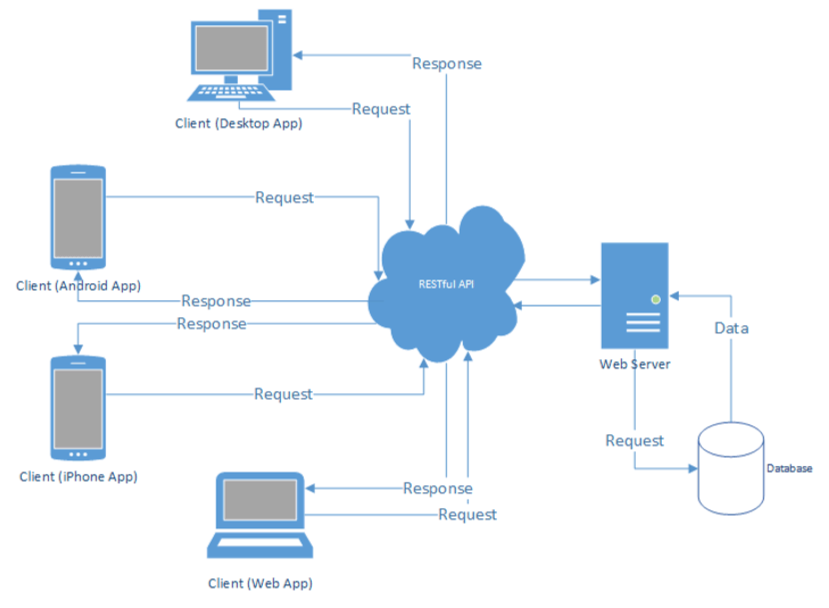
\includegraphics[scale=0.45]{chap1.images/rest-api-flow.png}
              \caption{REST API}
              \label{RESTAPI}
          \end{figure}

\end{itemize}


%__________________________________________________________________________________________________________
\newpage
\subsection{Environnement matériel}
\noindent Le tableau 1.1 montre les caractéristiques techniques des machines utilisées pour la réalisation de notre application.
\bigskip
\begin{table}[htbp]
    \renewcommand{\arraystretch}{1.9}
    \centering
    \begin{tabular}{|c|c|c|}
        \hline
        Ordinateur             & ASUS TUF F15 & ASUS TUF F15     \\
        \hline
        Propriétaire           & Balti Firas  & Mimouni Med Aziz \\
        \hline
        RAM                    & 32 GO        & 32 GO            \\
        \hline
        Processeur             & i5 11éme     & i5 11éme         \\
        \hline
        Système d’exploitation & Windows 11   & windows 11       \\
        \hline
    \end{tabular}
    \bigskip
    \caption{Description des machines de développement utilisées}

\end{table}
%____________________________________________________________________________________________
\subsection{ Environnement logiciel }

\noindent Les logiciels utilisés pour l’implémentation de notre solution sont les suivants sont les suivants :

\begin{itemize}
    \item[$\bullet$] \textbf{ Figma  :}
          C'est un outil de conception d’interface utilisateur (UI) et d’expérience utilisateur (UX) en ligne. Il permet aux designers de créer des designs d’interface utilisateur . Figma est également utilisé pour collaborer en temps réel. Nous l’avons utilisé dans notre projet pour concevoir les maquettes et les diagrammes de notre application.

          \begin{figure}[ht]
              \centering 
\includegraphics[scale=0.07]{chap1.images/FigmaLogo.png}
              \caption{Figma}
              \label{Figma}
          \end{figure}



    \item[$\bullet$] \textbf{ Android Studio :}
          C'est un environnement de développement intégré (IDE) développé par Google pour la création d’applications Android. Il est disponible gratuitement pour les développeurs Android. Nous l’avons utilisé dans notre cas pour bénéficier d’un émulateur android servant à débeuguer notre application.

          \begin{figure}[ht]
              \centering 
\includegraphics[scale=0.3]{chap1.images/andoird studio.png}
              \caption{Android Studio}
              \label{Android Studio}
          \end{figure}



    \item[$\bullet$] \textbf{  Overleaf :}
          C'est un éditeur en ligne de LaTeX, un langage de composition de documents scientifiques et techniques. Il permet aux utilisateurs de créer, de modifier et de collaborer sur des documents LaTeX en temps réel, Tout au long de notre stage de projet de fin d’étude, nous l’avons utilisé pour travailler ensemble sur un seul document et suivre les modifications apportées par chacune de nous en temps réel.

          \begin{figure}[h]
              \centering 
\includegraphics[scale=0.14]{chap1.images/overleaflogo.png}
              \caption{Overleaf}
              \label{fig: Overleaf}
          \end{figure}


          \bigskip
    \item[$\bullet$] \textbf{  Spyder :}
          C'est un environnement de développement interactif (IDE) spécialement conçu pour Python, offrant une interface conviviale et des fonctionnalités avancées telles que l'édition de code, l'exploration de variables et la gestion de projets. Nous avons choisi d'utiliser Spyder dans notre cas pour sa simplicité d'utilisation et sa compatibilité avec Python, ce qui nous a permis de développer et de déboguer efficacement notre code .


          \begin{figure}[ht]
              \centering
\includegraphics[scale=0.3]{chap1.images/spyder_logo.png}
              \caption{Spyder}
              \label{Spyder}
          \end{figure}
          \bigskip
    \item[$\bullet$] \textbf{  Jira :}
          C'est un outil de gestion de projet, conçu pour aider les équipes à planifier, suivre et gérer leurs tâches et leurs projets. Il offre une interface conviviale pour la création de backlogs, l'attribution de tâches, le suivi des progrès et la gestion des délais. Grâce à ses fonctionnalités de collaboration , Jira permet aux équipes de travailler de manière coordonnée et de respecter les délais de manière transparent.

          \begin{figure}[H]
              \centering
\includegraphics[scale=0.2]{chap1.images/jira-logo.png}
              \caption{Jira}

          \end{figure}

          \newpage

    \item[$\bullet$] \textbf{  Slack :}
          C'est une plateforme de communication collaborative propriétaire (SaaS). Nous avons utilisé Slack lors de notre période de stage pour assurer et faciliter la communication avec l’équipe de l’entreprise d’acceuil.

          \begin{figure}[ht]
              \centering
\includegraphics[scale=0.22]{chap1.images/Slack.logo.png}
              \caption{Slack}

          \end{figure}



    \item[$\bullet$] \textbf{  Material UI :}
          C'est une bibliothèque de composants React qui facilite la création d'interfaces utilisateurs avec des éléments préconçus basés sur les principes du Material Design de Google. Elle permet une personnalisation poussée et un développement rapide.
          \bigskip
          \begin{figure}[ht]
              \centering
\includegraphics[width=0.15\textwidth,height=1.8cm]{chap1.images/material-ui-logo.png}
              \caption{Material UI}

          \end{figure}

    \item[$\bullet$] \textbf{ Visme :}
          C'une plateforme de création visuelle en ligne,  nous avons utilisé cette outil pour la création de nos burndown charts.

          \begin{figure}[ht]
              \centering
\includegraphics[scale=0.3]{chap1.images/vismelogo.jpg}
              \caption{Visme}
          \end{figure}


    \item[$\bullet$] \textbf{ Postman :}
          C'est un outil qui simplifie le test et le développement d'API en permettant d'envoyer des requêtes HTTP et d'analyser les réponses via une interface utilisateur conviviale.

          \begin{figure}[H]
              \centering
\includegraphics[scale=0.28]{chap1.images/Postman-Logo.jpg}
              \caption{Postman}

          \end{figure}




\end{itemize}
%_________________________________________________________________________________________________________
%____________________________________________________________________________________________________________


\newpage
\section{Organisation du travail}

Pour assurer une organisation optimale tout au long du développement de notre projet, nous avons mis en place une série de processus et de pratiques collaboratives. Nous avons débuté par des séances de brainstorming, où nous avons généré et partagé des idées. Ces propositions ont ensuite été soumises à des réunions quotidiennes avec notre encadrant professionnel pour validation et conseils. En parallèle, nous avons consulté notre encadrant académique pour le filtrage et le développement des idées. Une fois la phase de conception achevée, nous avons entamé la création du backlog sur Jira, ce qui nous a permis de planifier et d'organiser efficacement les différentes tâches à réaliser. Ensuite, nous avons progressé vers la phase de codage.\\

\begin{figure}[ht]
    \centering
    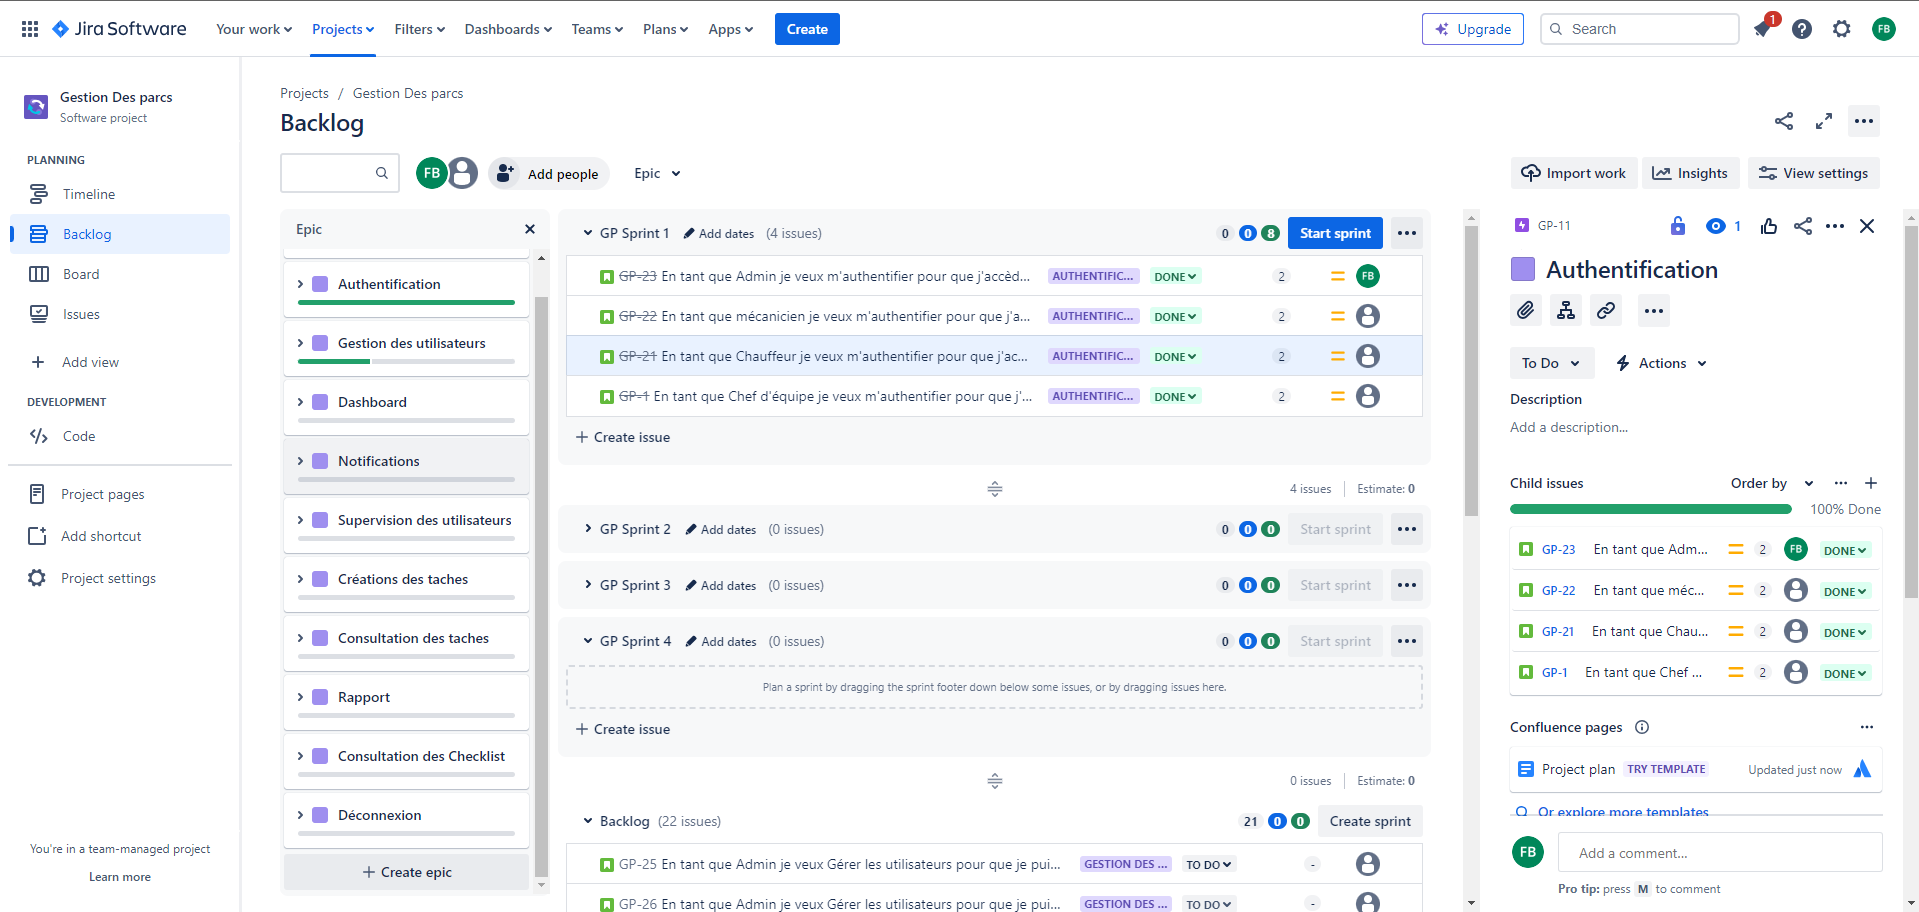
\includegraphics[width=0.85\textwidth]{chap1.images/jira.png}
    \caption{Création du backlog avec Jira}
\end{figure}

Pour faciliter la collaboration et le partage du code en temps réel, nous avons opté pour l'utilisation de GitHub. Chacun de nous a pu "pusher" ses changements une fois les tâches accomplies, ce qui nous a permis de suivre l'avancement de chacun et de garantir le respect des délais de réalisation de nos sprints. \\
\begin{figure}[ht]
    \centering
    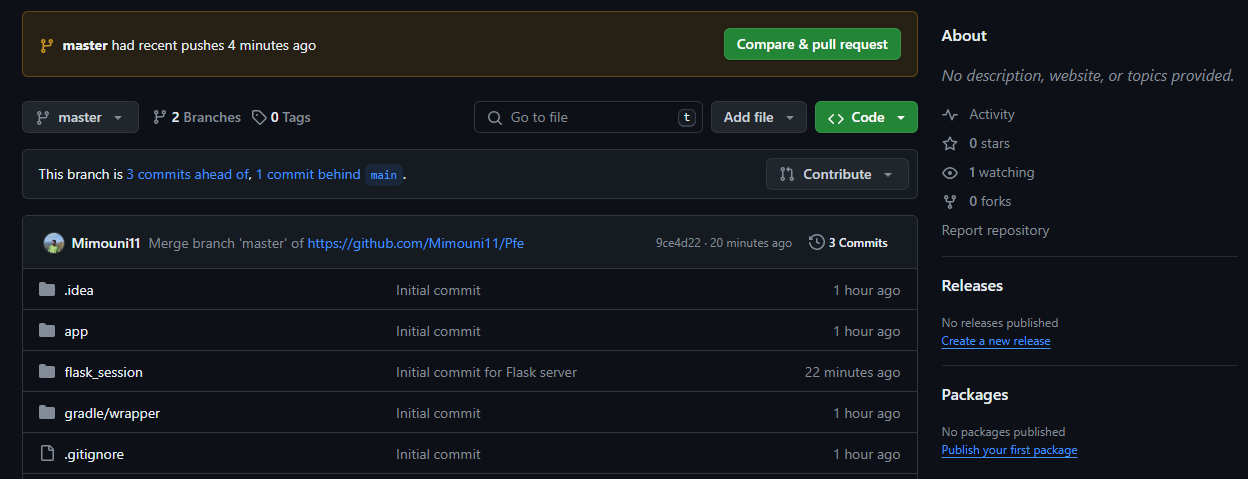
\includegraphics[width=0.85\textwidth]{chap1.images/depot git.png}

    \caption{Dépôt GitHub}
\end{figure}


%_____________________________________________________________________________________________________


\newpage
\section*{Conclusion}
\addcontentsline{toc}{section}{Conclusion}
\bigskip
\begin{sloppypar}
    Dans ce chapitre, nous avons introduit l’organisme d’accueil, clarifié le cadre du projet  et décrit les choix méthodologiques ainsi que l’architecture. Le prochain chapitre se concentrera sur la planification du projet et la définition des fonctionnalités de l’application
\end{sloppypar}








